\section{Results}
The 410 images of the database were preprocessed and segmented according to the methods described above, resulting in 6376 regions. Those segmented regions were compared to the groundtruth for labeling. A region was considered positive if the Dice Similarity Index between the candidate and the groundtruth was equal or higher than 0.2. This resulted in 110 regions labeled as positive (out of 115 masses in the groundtruth - 95.6\% of the total) and 6266 regions labeled as negative (15.28 negative regions per image).

The results of classification using the features of these regions can be seen in Table~\ref{class-results}, showing both the SVM and RF classifiers. The corresponding FROC curves can be found in Figs.~\ref{fig:res_lbp}-\ref{fig:res_no_lbp}.

\begin{table}[]
\centering
\caption{Results of mass detection for the two classifiers}
\label{class-results}
\begin{tabular}{llll} \\ [-1.75ex]
\hline \\ [-1.75ex]
\textbf{Features} & \textbf{Classifier} & \textbf{\begin{tabular}[c]{@{}l@{}}Partial\\ Area FROC\end{tabular}} & \textbf{\begin{tabular}[c]{@{}l@{}}TPR\\ at FPPI = 1\end{tabular}} \\ [1.75ex] \hline \\ [-1.75ex]
All               & SVM                 & 0.31                                                                 & 0.47                                                               \\
All               & RF                  & 0.13                                                                 & 0.21                                                               \\
No LBP            & SVM                 & 0.58                                                                 & 0.75                                                               \\
No LBP            & RF                  & 0.59                                                                 & 0.75                                                               \\ [1.5ex] \hline \\ [-1.75ex]
\multicolumn{4}{l}{\textit{Partial area FROC for FPPI between 0 and 1}}                                                                                                            
\end{tabular}
\end{table}
    
\begin{figure}[htb]
\caption{FROC Curve using all features including LBP comparing the RF and SVM classifiers.}
\begin{minipage}[b]{1.0\linewidth}
  \centering
  \centerline{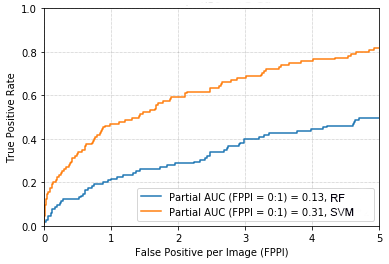
\includegraphics[width=8.5cm]{rf_svm_roc_lbp.png}}
%  \vspace{2.0cm}
\end{minipage}
  \label{fig:res_lbp}
\end{figure}
    
\begin{figure}[htb]
\caption{FROC Curve using all features except LBP comparing the RF and SVM classifiers.}
\begin{minipage}[b]{1.0\linewidth}
  \centering
  \centerline{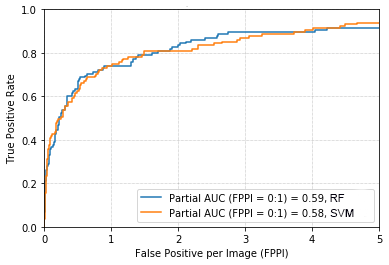
\includegraphics[width=8.5cm]{rf_svm_roc.png}}
%  \vspace{2.0cm}
\end{minipage}
 \label{fig:res_no_lbp}
\end{figure}
